\chapter{Implementacja}
\label{chapter:implementation}

\section{Kontrola wersji}

Do przechowywania kodu źródłowego projektu Ebook-Wizard wykorzystywany jest system kontroli wersji Git oraz serwis hostingowy GitHub. Dzięki zastosowaniu systemu kontroli wersji możliwe jest śledzenie zmian w kodzie, zarządzanie różnymi wersjami projektu oraz ewentualna współpraca zespołowa nad kodem. \cite{pro_git}

Wybór systemu kontroli wersji Git został dokonany ze względu na powszechność tego rozwiązania. Jak podają statystyki opracowane przez członka zespołu odpowiedzialnego za rozwój serwisu Stack Overflow, w 2023 roku Git był wykorzystywany aż przez 93\% ankietowanych programistów. \cite{git_usage_stats}

Struktura katalogów w repozytorium projektu Ebook-Wizard wygląda następująco:
\begin{itemize}
    \item folder \verb|.github| - konfiguracja usługi GitHub Actions (patrz: Rozdział \ref{chapter:ci}),
    \item folder \verb|backend| - pełny kod źródłowy serwera backendowego,
    \item folder \verb|docs| - kopia niniejszego dokumentu w formacie LaTeX,
    \item folder \verb|frontend| - pełny kod źródłowy serwera frontendowego,
    \item folder \verb|infra| - skrypty Terraform umożliwiające automatyzację tworzenia usług sieciowych w chmurze Amazon Web Services,
    \item folder \verb|scripts| - dodatkowe skrypty wykorzystywane pomocniczo w procesie implementacji.
\end{itemize}

\section{Baza danych}

\subsection{Wybór bazy danych}

Do przechowywania danych o e-bookach została wybrana nierelacyjna baza danych MongoDB. Wybór ten został dokonany ze względu na korzystny plan finansowy. Twórcy bazy MongoDB oferują usługę MongoDB Atlas, która pozwala na utworzenie darmowej bazy danych o rozmiarze do 512 MB. Ponadto, MongoDB jest bardzo wydajne i pozwala na przechowywanie złożonych struktur bez konieczności definiowania osobnej tabeli dla każdego typu obiektu. \cite{mongodb_book}

MongoDB jest tzw. bazą dokumentową, do której zapisywane są obiekty w formacie~JSON. Jej dużą zaletą jest możliwość zagnieżdżania jednego typu obiektu w drugim, co likwiduje konieczność wykonywania kosztownych operacji \verb|JOIN|, które wykorzystywane są w konkurencyjnych bazach SQL. \cite{aws_mongodb_vs_sql}

Wadą MongoDB jest natomiast brak wymuszania więzów integralności, co jest spowodowane brakiem mechanizmu kluczy obcych. Relacje pomiędzy poszczególnymi obiektami w MongoDB można tworzyć na przykład poprzez zagnieżdżanie jednych obiektów w drugich, albo poprzez zarządzanie relacjami na poziomie aplikacji. \cite{mongodb_book} Obie te metody są wykorzystywane w bazie serwisu Ebook-Wizard.

\subsection{Projekt bazy danych}

Cechą charakterystyczną MongoDB jest podział bazy na tzw. kolekcje. W przypadku tradycyjnych baz SQL, bazę danych dzieli się na tabele, które mają wiersze i kolumny. W przypadku MongoDB, bazę danych dzieli się na kolekcje, do których zapisuje się powiązane ze sobą obiekty. \cite{aws_mongodb_vs_sql}

W bazie projektu Ebook-Wizard zdefiniowano następujące kolekcje:

\begin{itemize}
    \item \verb|EbookFile| - kolekcja przechowująca informacje na temat plików zaimportowanych przez użytkownikow,
    \item \verb|EbookProject| - kolekcja przechowująca informacje na temat projektów utworzonych przez użytkowników,
    \item \verb|EbookFileBookmark| - kolekcja przechowująca zakładki utworzone przez użytkowników,
    \item \verb|QueueTask| - przechowuje identyfikatory zadań dodanych do kolejki; więcej o tym mechaniźmie można przeczytać w rodziale \ref{subsection:queue_backend}.
\end{itemize}

MongoDB nie wymusza, aby obiekty przechowywane w jednej kolekcji miały tą samą strukturę, \cite{mongodb_book} jednakże w Ebook-Wizard zdecydowana większość zapisywanych do bazy obiektów posiada sformalizowaną, jednolitą strukturę. W tabelach \ref{tab:ebook_file_db_struct}, \ref{tab:ebook_project_db_struct}, \ref{tab:ebook_file_bookmark_db_struct} oraz \ref{tab:queue_task_db_struct} przedstawiono strukturę danych zapisywanych w poszczególnych kolekcjach bazodanowych.

Na Rysunku \ref{list:db_scheme_diagram} przedstawiono schemat bazy danych w formie graficznej. Linią ciągłą zaznaczono obiekty zapisywane bezpośrednio do odpowiednich kolekcji bazy MongoDB jako dokumenty najwyższego poziomu (\verb|EbookProject|, \verb|EbookFile|, \verb|QueueTask|, \verb|EbookFileBookmark|). Linią przerywaną oznaczone są obiekty, które wchodzą w skład innych obiektów, natomiast linią kropkowaną oznaczono typy wyliczeniowe.

Należy zwrócić uwagę, że pomiędzy obiektami \verb|EbookFileBookmark| oraz \verb|EbookFile| nie ma zaznaczonej relacji z uwagi na specyfikę bazy MongoDB. Baza MongoDB jest bazą nierelacyjną, co oznacza, że relacje w niej są umowne, niewymuszane przez silnik bazodanowy. Typ \verb|EbookFileBookmark| zawiera w sobie identyfikator do typu \verb|EbookFile|, jednakże integralność tej relacji nie jest kontrolowana przez MongoDB, i musi być zapewniona przez programistę w trakcie implementacji aplikacji. \cite{mongodb_book}

\begin{table}
    \caption{Opis struktury typu EbookFile}
    \renewcommand{\arraystretch}{1.3} % Ustawienie minimalnej wysokości rzędu
    \centering
    \begin{tabular}{|>{\centering\arraybackslash}m{4.7cm}|>{\centering\arraybackslash}m{4.7cm}|>{\centering\arraybackslash}m{4.7cm}|} \hline
        \textbf{Nazwa pola} & \textbf{Opis typu pola} & \textbf{Opis pola} \\ \hline
        \verb|id| & wartość tekstowa & unikalny identyfikator generowany przez MongoDB \\ \hline
        \verb|ownerUserId| & wartość tekstowa & identyfikator użytkownika wygenerowany przez usługę Amazon Cognito \\ \hline
        \verb|name| & wartość tekstowa & nazwa e-booka  \\ \hline
        \verb|author| & wartość tekstowa & autor e-booka \\ \hline
        \verb|description| & wartość tekstowa & opis e-booka \\ \hline
        \verb|containerNameKey| & wartość tekstowa & nazwa folderu w którym jest przechowywany e-book \\ \hline
        \verb|coverImageKey| & wartość tekstowa & identyfikator pliku okładki w usłudze Amazon S3; może być pusty \\ \hline
        \verb|tags| & kolekcja wartości tekstowych & lista tagów e-booka \\ \hline
        \verb|creationDate| & data & data i godzina utworzenia pliku w bazie \\ \hline
        \verb|isPublic| & wartość logiczna & informacja o udostępnieniu e-booka \\ \hline
        \verb|conversionSourceFormat| & jedna z wartości: EPUB, MOBI, TXT, AZW3, HTML, HTML, PDF & format używany do wykonywania konwersji na inne formaty \\ \hline
        \verb|editLock| & obiekt typu \verb|EbookEditLock|\newline(tabela \ref{tab:ebook_edit_lock_db_struct}) & obiekt zagnieżdżony, informuje o tym, czy plik jest zablokowany do modyfikacji \\ \hline
        \verb|downloadableFiles| & kolekcja obiektów \verb|EbookDownloadable-| \verb|Resource|\newline(Tabela \ref{tab:ebook_downloadable_resource_db_struct}) & obiekty zagnieżdżone, informacja o rewizjach pliku \\ \hline
        \verb|totalSizeBytes| & wartość liczbowa & łączny rozmiar pliku, wykorzystywany do ustalenia wykorzystania limitu dyskowego \\ \hline
    \end{tabular}
    \label{tab:ebook_file_db_struct}
\end{table}

\begin{table}
    \caption{Opis struktury typu EbookProject}
    \renewcommand{\arraystretch}{1.3} % Ustawienie minimalnej wysokości rzędu
    \centering
    \begin{tabular}{|>{\centering\arraybackslash}m{4.7cm}|>{\centering\arraybackslash}m{4.7cm}|>{\centering\arraybackslash}m{4.7cm}|} \hline
        \textbf{Nazwa pola} & \textbf{Opis typu pola} & \textbf{Opis pola} \\ \hline
        \verb|id| & wartość tekstowa & unikalny identyfikator generowany przez MongoDB \\ \hline
        \verb|ownerUserId| & wartość tekstowa & identyfikator użytkownika wygenerowany przez usługę Amazon Cognito \\ \hline
        \verb|name| & wartość tekstowa & nazwa e-booka  \\ \hline
        \verb|author| & wartość tekstowa & autor e-booka \\ \hline
        \verb|description| & wartość tekstowa & opis e-booka \\ \hline
        \verb|containerNameKey| & wartość tekstowa & nazwa folderu w którym jest przechowywany e-book \\ \hline
        \verb|coverImageKey| & wartość tekstowa & identyfikator pliku okładki w usłudze Amazon S3; może być pusty \\ \hline
        \verb|tags| & kolekcja wartości tekstowych & lista tagów e-booka \\ \hline
        \verb|creationDate| & data & data i godzina utworzenia pliku w bazie \\ \hline
        \verb|isPublic| & wartość logiczna & informacja o udostępnieniu e-booka \\ \hline
        \verb|lock| & obiekt typu \verb|EbookEditLock|\newline(Tabela \ref{tab:ebook_edit_lock_db_struct}) & obiekt zagnieżdżony, informuje o tym, czy plik jest zablokowany do modyfikacji \\ \hline
        \verb|illustrations| & kolekcja obiektów \verb|EbookProject-| \verb|Illustration|\newline(Tabela \ref{tab:ebook_project_illustration_db_struct}) & lista plików graficznych osadzonych w projekcie \\ \hline
        \verb|downloadableFiles| & kolekcja obiektów \verb|EbookDownloadable| \verb|Resource|\newline(Tabela \ref{tab:ebook_downloadable_resource_db_struct}) & lista dostępnych do pobrania wersji projektu \\ \hline
        \verb|chapters| & kolekcja obiektów \verb|EbookProjectChapter|\newline(Tabela \ref{tab:ebook_project_chapter_db_struct}) & lista rozdziałów zdefiniowanych w projekcie \\ \hline
        \verb|totalSizeBytes| & wartość liczbowa & łączny rozmiar projektu, wykorzystywany do ustalenia wykorzystania limitu dyskowego \\ \hline
    \end{tabular}
    \label{tab:ebook_project_db_struct}
\end{table}

\begin{table}
    \caption{Opis struktury typu EbookFileBookmark}
    \renewcommand{\arraystretch}{1.3} % Ustawienie minimalnej wysokości rzędu
    \centering
    \begin{tabular}{|>{\centering\arraybackslash}m{4.7cm}|>{\centering\arraybackslash}m{4.7cm}|>{\centering\arraybackslash}m{4.7cm}|} \hline
        \textbf{Nazwa pola} & \textbf{Opis typu pola} & \textbf{Opis pola} \\ \hline
        \verb|id| & wartość tekstowa & unikalny identyfikator generowany przez MongoDB \\ \hline
        \verb|ebookFileId| & wartość tekstowa & identyfikator e-booka, do którego przypisane są zakładki \\ \hline
        \verb|userId| & wartość tekstowa & identyfikator użytkownika, który utworzył zakładki  \\ \hline
        \verb|bookmarkedPages| & kolekcja wartości liczbowych & numery stron (indeksowane od 1), na których założono zakładki \\ \hline
    \end{tabular}
    \label{tab:ebook_file_bookmark_db_struct}
\end{table}

\begin{table}
    \caption{Opis struktury typu QueueTask}
    \renewcommand{\arraystretch}{1.3} % Ustawienie minimalnej wysokości rzędu
    \centering
    \begin{tabular}{|>{\centering\arraybackslash}m{4.7cm}|>{\centering\arraybackslash}m{4.7cm}|>{\centering\arraybackslash}m{4.7cm}|} \hline
        \textbf{Nazwa pola} & \textbf{Opis typu pola} & \textbf{Opis pola} \\ \hline
        \verb|id| & wartość tekstowa & unikalny identyfikator generowany przez MongoDB \\ \hline
        \verb|queueName| & wartość tekstowa & identyfikator kolejki w systemie AWS SQS \\ \hline
        \verb|taskPayload| & wartość tekstowa & dodatkowy obiekt dołączony do zakolejkowanego zadania  \\ \hline
        \verb|status| & jedna z wartości: \verb|IN_QUEUE|, \verb|IN_PROGRESS|, \verb|COMPLETED|, \verb|FAILED| & informacja o aktualnym statusie zadania \\ \hline
        \verb|creationDate| & wartość tekstowa & data i godzina dodania zadania do kolejki \\ \hline
    \end{tabular}
    \label{tab:queue_task_db_struct}
\end{table}

\begin{table}
    \caption{Opis struktury typu zagnieżdżonego EbookDownloadableResource}
    \renewcommand{\arraystretch}{1.3} % Ustawienie minimalnej wysokości rzędu
    \centering
    \begin{tabular}{|>{\centering\arraybackslash}m{4.7cm}|>{\centering\arraybackslash}m{4.7cm}|>{\centering\arraybackslash}m{4.7cm}|} \hline
        \textbf{Nazwa pola} & \textbf{Opis typu pola} & \textbf{Opis pola} \\ \hline
        \verb|stub| & wartość tekstowa & unikalny identyfikator wygenerowany przez serwer backendowy \\ \hline
        \verb|format| & jedna z wartości: EPUB, MOBI, TXT, AZW3, HTML, HTML, PDF & format, w którym został zapisany dany zasób \\ \hline
        \verb|creationDate| & data & data utworzenia zasobu  \\ \hline
        \verb|fileKey| & wartość tekstowa & identyfikator pliku w usłudze Amazon S3 \\ \hline
    \end{tabular}
    \label{tab:ebook_downloadable_resource_db_struct}
\end{table}

\begin{table}
    \caption{Opis struktury typu zagnieżdżonego EbookEditLock}
    \renewcommand{\arraystretch}{1.3} % Ustawienie minimalnej wysokości rzędu
    \centering
    \begin{tabular}{|>{\centering\arraybackslash}m{4.7cm}|>{\centering\arraybackslash}m{4.7cm}|>{\centering\arraybackslash}m{4.7cm}|} \hline
        \textbf{Nazwa pola} & \textbf{Opis typu pola} & \textbf{Opis pola} \\ \hline
        \verb|isLocked| & wartość logiczna & informacja o tym, czy edycja zasobu jest aktualnie zablokowana \\ \hline
        \verb|lockExpirationDate| & data & data automatycznego zwolnienia blokady \\ \hline
    \end{tabular}
    \label{tab:ebook_edit_lock_db_struct}
\end{table}

\begin{table}
    \caption{Opis struktury typu zagnieżdżonego EbookProjectChapter}
    \renewcommand{\arraystretch}{1.3} % Ustawienie minimalnej wysokości rzędu
    \centering
    \begin{tabular}{|>{\centering\arraybackslash}m{4.7cm}|>{\centering\arraybackslash}m{4.7cm}|>{\centering\arraybackslash}m{4.7cm}|} \hline
        \textbf{Nazwa pola} & \textbf{Opis typu pola} & \textbf{Opis pola} \\ \hline
        \verb|id| & wartość tekstowa & unikalny identyfikator generowany przez MongoDB \\ \hline
        \verb|name| & wartość tekstowa & nazwa rozdziału zdefiniowana przez użytkownika \\ \hline
        \verb|contentHtml| & wartość tekstowa & treść rozdziału w formacie HTML  \\ \hline
        \verb|creationDate| & data & data i godzina utworzenia rozdziału \\ \hline
        \verb|lastModifiedDate| & wartość tekstowa & data i godzina zmodyfikowania rozdziału \\ \hline
    \end{tabular}
    \label{tab:ebook_project_chapter_db_struct}
\end{table}

\begin{table}
    \caption{Opis struktury typu zagnieżdżonego EbookProjectIllustration}
    \renewcommand{\arraystretch}{1.3} % Ustawienie minimalnej wysokości rzędu
    \centering
    \begin{tabular}{|>{\centering\arraybackslash}m{4.7cm}|>{\centering\arraybackslash}m{4.7cm}|>{\centering\arraybackslash}m{4.7cm}|} \hline
        \textbf{Nazwa pola} & \textbf{Opis typu pola} & \textbf{Opis pola} \\ \hline
        \verb|stub| & wartość tekstowa & unikalny identyfikator ilustracji wygenerowany przez serwer backendowy \\ \hline
        \verb|fileKey| & wartość tekstowa & identyfikator pliku graficznego w usłudze Amazon S3 \\ \hline
    \end{tabular}
    \label{tab:ebook_project_illustration_db_struct}
\end{table}

\begin{figure}[h]
    \centering
    \setlength{\fboxsep}{0pt}
    \setlength{\fboxrule}{0.4pt}
    \includesvg[width=0.9\textwidth]{chap5/app-db-scheme.drawio.svg}
    \caption{Schemat bazy danych}
    \label{list:db_scheme_diagram}
\end{figure}

\section{Serwer backend}

\subsection{Zasada działania}

Serwer backendowy, obok klienta frontendowego, jest jednym z dwóch komponentów serwisu Ebook-Wizard. Serwer backendowy jest serwerem HTTP, który nieustannie nasłuchuje żądań wysyłanych przez przeglądarkowego klienta frontend.

Gdy nadejdzie żądanie HTTP, serwer backendowy analizuje żądanie i podejmuje odpowiednią akcję, na przykład utworzenie e-booka w bazie lub rozpoczęcie procedury konwersji pliku. Żądanie musi być odpowiednio uwierzytelnione (patrz: Rozdział \ref{subsection:authn_authz}), aby udowodnić tożsamość osoby wysyłającej.

Dane pomiędzy serwerem backendowym a klientem są przesyłane w formacie JSON. Format ten został wybrany ze względu na czytelność oraz zwięzłość zapisu.

Obecnie istnieje tylko jeden klient, klient frontendowy uruchamiany w przeglądarce, jednak dzięki wydzieleniu backendu jako osobnego serwera, możliwe jest dodanie w przyszłości na przykład aplikacji mobilnej.

\subsection{Wykorzystane technologie}

Do zaimplementowania serwera backendowego został wykorzystany język programowania Java oraz framework Spring. \cite{spring_in_action_book} Do pobierania bibliotek oraz przeprowadzania procesu kompilacji wykorzystany został program Maven. \cite{maven_guide} Poniżej zaprezentowana została lista wykorzystywanych bibliotek, wraz z krótkim opisem przeznaczenia każdej biblioteki.

\begin{itemize}
    \item \textbf{Lombok}\hspace{0.6em}-\hspace{0.6em}zmniejsza objętość kodu źródłowego przez dodanie adnotacji generujących powtarzalne fragmenty kodu.
    \item \textbf{Spring Data MongoDB}\hspace{0.6em}-\hspace{0.6em}umożliwia połączenie z bazą danych MongoDB.
    \item \textbf{Jakarta Mail API}\hspace{0.6em}-\hspace{0.6em}umożliwia wysyłanie wiadomości e-mail.
    \item \textbf{Spring Security}\hspace{0.6em}-\hspace{0.6em}wymagane do konfiguracji uwierzytelniania.
    \item \textbf{Spring Boot Bean Validation}\hspace{0.6em}-\hspace{0.6em}dodaje adnotacje umożliwiające walidację danych przesyłanych przez klienta.
    \item \textbf{Spring Web}\hspace{0.6em}-\hspace{0.6em}umożliwia pracę aplikacji jako serwer HTTP.
    \item \textbf{Spring Boot Configuration Processor}\hspace{0.6em}-\hspace{0.6em}wspiera możliwość konfigurowania aplikacji przy użyciu plików \verb|.properties|.
    \item \textbf{JUnit},\hspace{0.6em}\textbf{AssertJ},\hspace{0.6em}\textbf{Mockito}\hspace{0.6em}-\hspace{0.6em}biblioteki używane do uruchamiania testów jednostkowych.
    \item \textbf{Spring Cloud AWS}\hspace{0.6em}-\hspace{0.6em}umożliwia działanie bibliotek integracji z usługami firmy Amazon.
    \item \textbf{Spring Cloud AWS SQS}\hspace{0.6em}-\hspace{0.6em}dodaje integrację z usługą kolejkowania Amazon SQS.
    \item \textbf{Spring Cloud AWS SES}\hspace{0.6em}-\hspace{0.6em}kodaje integrację z usługą wysyłania e-maili Amazon SES.
    \item \textbf{Spring Cloud AWS S3}\hspace{0.6em}-\hspace{0.6em}dodaje integrację z usługą przechowywania plików Amazon S3.
    \item \textbf{Apache Tika}\hspace{0.6em}-\hspace{0.6em}biblioteka pozwalają na wykrywanie typu pliku na podstawie jego zawartości.
    \item \textbf{Twelvemonkeys ImageIO}\hspace{0.6em}-\hspace{0.6em}odpowiada za konwertowanie plików graficznych pomiędzy formatami.
    \item \textbf{Jsoup}\hspace{0.6em}-\hspace{0.6em}wymagany do konwersji obiektów Java do postaci kodu JSON.
    \item \textbf{Epubify}\hspace{0.6em}-\hspace{0.6em}biblioteka umożliwiająca tworzenie plików epub poprzez podanie zawartości e-booka w formacie html.
    \item \textbf{AWS SDK Amazon Polly}\hspace{0.6em}-\hspace{0.6em}klient usługi syntezy głosu Amazon Polly.
    \item \textbf{AWS SDK Cognito Identity}\hspace{0.6em}-\hspace{0.6em}dostarcza interakcję z usługą uwierzytelniania Amazon Cognito.
\end{itemize}

\subsection{Zależności systemowe}

Z uwagi na przenośność aplikacji napisanych w języku Java, backend Ebook-Wizard może być uruchomiony na dowolnym systemie operacyjnym, który umożliwia zainstalowanie środowiska uruchomieniowego Java. Istnieją jednak pewne zależności systemowe, które muszą być zainstalowane w systemie operacyjnym, aby backend działał poprawnie.

\begin{itemize}
    \item Pakiet \verb|calibre| - projekt Calibre dostarcza narzędzia, które mogą być wykorzystywane do konwertowania dokumentów między formatami takimi jak pdf, txt, epub, mobi. \cite{calibre_user_manual}
    \item Pakiet \verb|pandoc| - dostarcza narzędzia konwersji dla formatu html. \cite{pandoc_user_manual}
\end{itemize}

\subsection{Architektura MVC}
\label{subsection:mvc_architecture}

Zgodnie z konwencją aplikacji webowych pisanych we frameworku Spring, serwer backendowy zbudowany jest przy użyciu warstwowego modelu MVC \textit{(ang. Model View Controller)}. Jak podaje literatura, model MVC jest sposobem odseparowania poszczególnych warstw programu poprzez wprowadzenie warstwy danych (model), interfejsu użytkownika (widok) oraz kontroli przepływu danych i komunikacji z użytkownikiem (kontroler). \cite{spring_in_action_book}

W przypadku backendu Ebook-Wizard, interfejs użytkownika jest wydzielony do osobnej aplikacji uruchamianej w przeglądarce użytkownika. Widokami zwracanymi przez backend są więc pliki JSON, które są odpowiednio interpretowane i wyświetlane na ekranie przez frontend.

Pełny podział aplikacji na warstwy został przedstawiony na Rysunku \ref{fig:backend_layers}. Zgodnie z tym modelem, zapytanie przesłane przez użytkownika najpierw jest przekazywane do odpowiedniego kontrolera. Kontroler obsługujący żądanie jest wybierany przez biblioteki Spring na podstawie ścieżki zapytania HTTP. Następnie kontroler wywołuje odpowiednią metodę w obiekcie usługi (ang. service). Usługa wykonuje właściwą logikę operacji zleconej przez użytkownika. Wykonanie większości operacji wymaga komunikacji z bazą danych, a komunikacja ta odbywa się za pośrednictwem warstwy repozytorium. Usługa może odpytać repozytorium o dane z bazy, lub zlecić modyfikację rekordu w bazie. Po wykonaniu tej operacji, usługa zwraca rezultat operacji do kontrolera, a kontroler zwraca dane do użytownika. Framework Spring automatycznie konwertuje dane zwrócone przez kontroler do formatu JSON.

\begin{figure}[h]
    \centering
    \setlength{\fboxsep}{0pt}
    \setlength{\fboxrule}{0.4pt}
    \includesvg[width=0.9\textwidth]{chap5/backend-layers.drawio.svg}
    \caption{Architektura warstwowa serwera backendowego}
    \label{fig:backend_layers}
\end{figure}

Dla przykładu: użytkownik przesyła do backendu żądanie zwrócenia informacji o wykorzystaniu limitu pamięci dyskowej. Ponieważ ścieżka zapytania HTTP to \verb|/ebook/disk/usage|, framework Spring wykrywa na podstawie adnotacji umieszczonych w kodzie źródłowym, że należy wywołać metodę \verb|getUsageBytes()| z klasy \verb|EbookDiskUsageController|. Kontroler przyjmuje to zapytanie i decyduje, że należy odpytać metodę \verb|calculateDiskUsage()| znajdującą się w klasie (usłudze) \verb|EbookDiskUsageCalcService|. Ponieważ żądana operacja wymaga dostępu do bazy danych, usługa odpytuje repozytoria \verb|EbookProjectRepository| oraz \verb|EbookFileRepository| o zasoby z bazy MongoDB. Po obliczeniu łącznego rozmiaru wszystkich zasobów, usługa zwraca wyliczone informacje kontrolerowi, a kontroler użytkownikowi.

\subsection{Zdefiniowane kontrolery}

W kodzie źródłowym backendu Ebook-Wizard zdefiniowane jest 9 kontrolerów zdolnych do odbierania żądań użytkowników. 

\begin{enumerate}
    \item \verb|EbookFileController| - obsługa zarządzania plikami.
    \item \verb|EbookFileBookmarkController| - obsługa zarządzania zakładami utworzonymi w pliku.
    \item \verb|EbookProjectController| - obsługa zarządzania projektami.
    \item \verb|EbookDiskUsageController| - obsługa zwracania informacji o limicie pamięci dyskowej.
    \item \verb|EbookProjectChapterController| - obsługa zarządzania rozdziałami w projekcie.
    \item \verb|EbookAccountCleanupController| - zawiera metodę umożliwiającą wyczyszczenie wszystkich rekordów powiązanych z kontem.
    \item \verb|EbookWizardStatisticsController| - obsługa zwracania statystyk aplikacji.
    \item \verb|AudiobookGenerationController| - obsługa żądań syntezy głosu.
    \item \verb|QueueTaskTrackingController| - obsługa zwracania informacji o zakolejkowanych zadaniach.
\end{enumerate}

\subsection{Zarządzanie plikami}

Głównymi operacjami na plikach, które udostępnia backend, są: importowanie, modyfikacja metadanych, usuwanie, udostępnianie, konwersja na inny format pliku, konwersja na projekt oraz przesyłanie na czytnik. Ponadto, wspierane jest umieszczanie zakładek w plikach.

Wszystkie z powyższych operacji są obsługiwane przez kontroler \verb|EbookFileController|, za wyjątkiem operacji na zakładkach, które wydzielone są do osobnego kontrolera \verb|EbookFileBookmarkController|.

Importowanie odbywa się przez przesłanie zapytania HTTP zawierającego plik, który ma być zapisany w bazie Ebook-Wizard. Gdy użytkownik prześle plik, najpierw sprawdzane jest, czy użytkownik jest zalogowany i czy wykonanie operacji nie spowoduje przekroczenia limitu pamięci dyskowej. Następnie wykonywana jest detekcja typu przesłanego pliku przy użyciu biblioteki Apache Tika. Zapytania zawierające pliki o nierozpoznanym formacie są odrzucane. Następnie backend wykonuje próbę odczytania metadanych z pliku przesłanego przez użytkownika, co pozwala zapisać do bazy danych tytuł, imię i nazwisko autora, opis oraz tagi. Jeśli przesłany plik ma ustawiony obraz okładki, obraz zostaje wyodrębniony i przesłany do usługi Amazon S3. W wyniku tych operacji skonstruowany zostaje obiekt \verb|EbookFile|, który zostaje zapisany do bazy danych MongoDB przy użyciu dedykowanego repozytorium. Kod źródłowy operacji importowania został zaprezentowany na Rysunku \ref{listing:import_file_method}.

Konwersja pomiędzy formatami jest operacją kosztowną, zatem serwer nie wykonuje jej natychmiastowo, tylko przekazuje jej wykonanie do kolejki. Mechanizm kolejkowania został opisany w Rozdziale \ref{subsection:queue_backend}. Do wykonania konwersji wykorzystywane są narzędzia Calibre oraz Pandoc. Backend wywołuje te narzędzia poprzez uruchomienie odpowiedniej komendy jako podprocesu. Po wykonaniu konwersji backend przesyła wygenerowany plik do usługi Amazon S3 oraz zapisuje do bazy MongoDB informację o tym, że dostępna jest nowa wersja pliku.

Przesłanie pliku na czytnik opiera się na protokole e-mailowym. Klient przesyła do backendu informację o identyfikatorze pliku, docelowym adresie e-mail oraz o docelowym formacie pliku. Następnie backend przekazuje żądanie do usługi Amazon SES, która nadaje wiadomość e-mail. Producenci czytników e-booków, tacy jak Amazon Kindle, wystawiają specjalne adresy e-mailowe, które czytniki nieustannie nasłuchują, aby pobierać z nich przesyłane e-booki.

Modyfikacja metadanych również opiera się na wykorzystaniu narzędzia Calibre. Gdy użytkownik prześle żądanie zmiany metadanych, zmiana dokonywana jest najpierw w bazie danych MongoDB, a następnie przy pomocy Calibre we wszystkich formatach przypisanych do danej instancji obiektu \verb|EbookFile|.

\begin{figure}[h]
    \centering
    \setlength{\fboxsep}{0pt}
    \setlength{\fboxrule}{0.4pt}
    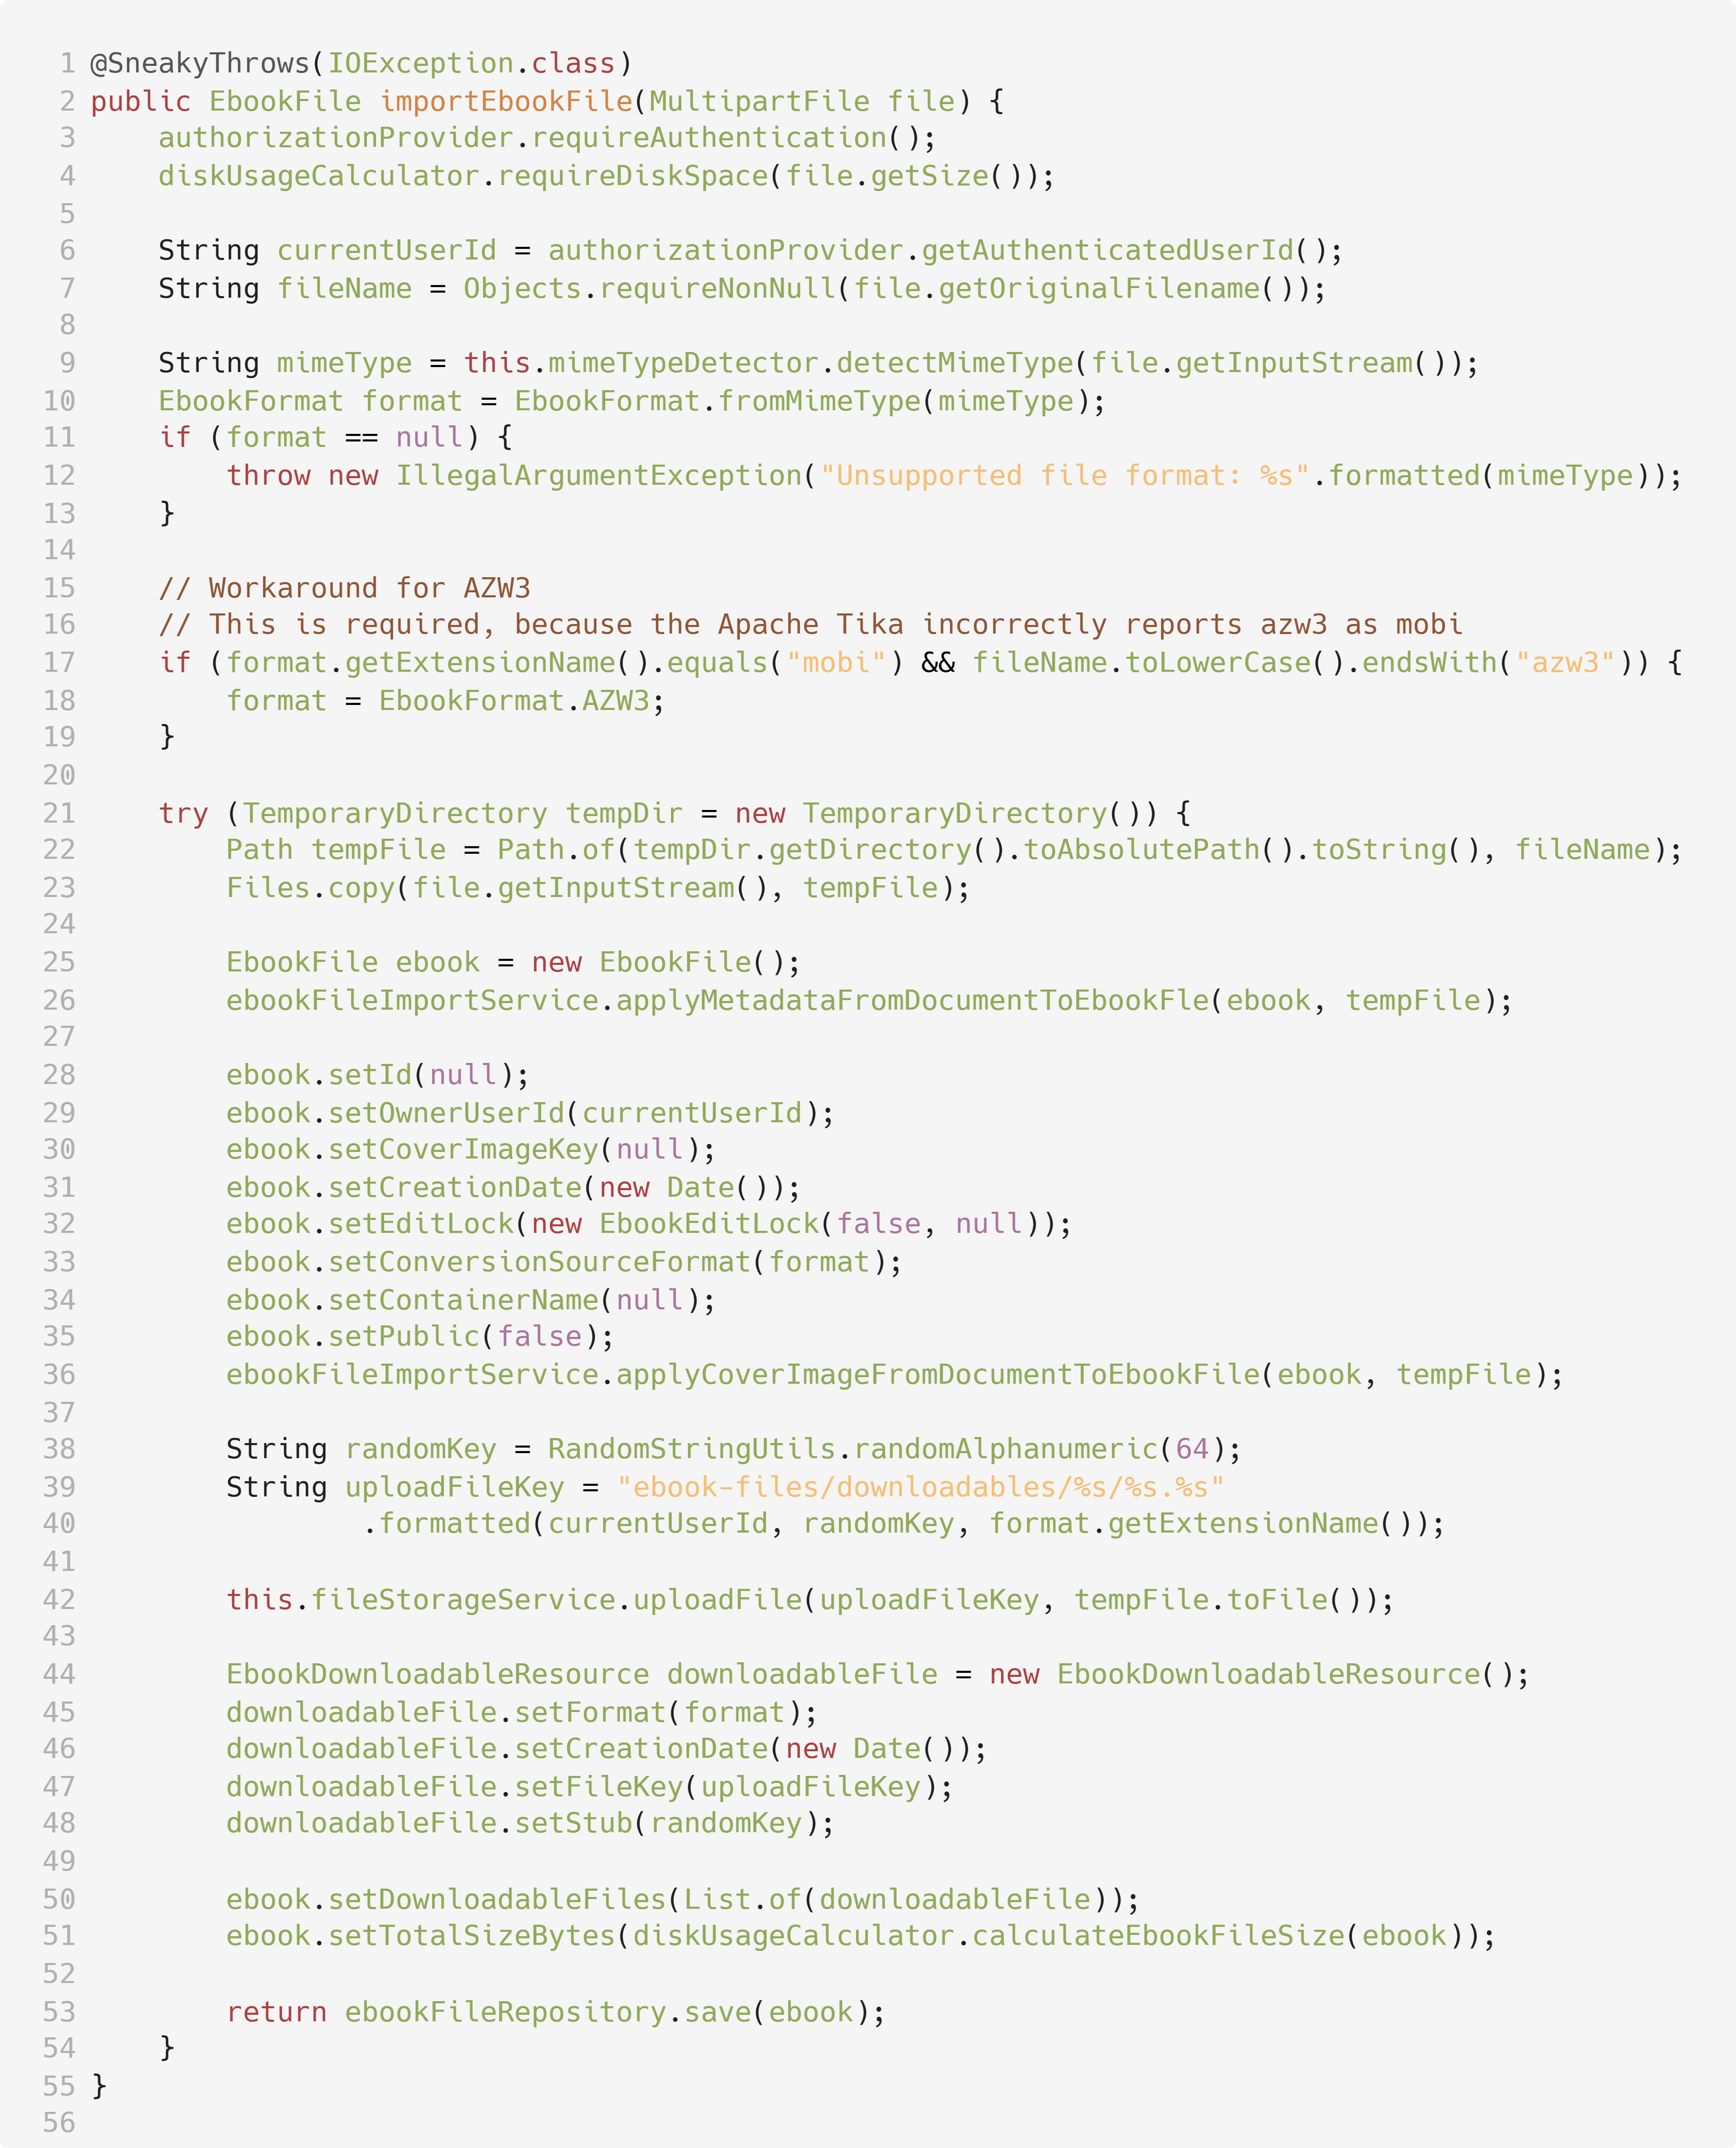
\includegraphics[width=0.8\textwidth]{chap5/import-file-listing.png}
    \caption{Kod źrodłowy metody importującej plik}
    \label{listing:import_file_method}
\end{figure}

\subsection{Zarządzanie projektami}

W przypadku projektów, głównymi wspieranymi operacjami jest tworzenie projektu, zmiana metadanych, konwersja projektu do pliku, usuwanie, udostępnianie oraz przesyłanie na czytnik oraz zarządzanie treścią i strukturą rozdziałów.

Projekty w kodzie źródłowym reprezentuje klasa \verb|EbookProject|. Posiada ona zbliżoną strukturę do typu \verb|EbookFile|, jednakże zamiast przechowywania wyłącznie referencji do plików w usłudze S3, przechowuje ona informacje o rozdziałach utworzonych w ramach danego projektu. Treść rozdziałów przechowywana jest bazie danych MongoDB w formie kodu html.

W celu wyeksportowania projektu (np. do formatu pdf) wykorzystywana jest biblioteka \verb|epubify|. Najpierw, treść projektu jest zapisywana do pliku o rozszerzeniu epub. Następnie, dokument epub konwertowany jest do docelowego formatu przy użyciu narzędzi dostarczanych przez Calibre. Dodatkowy krok pośredni w postaci konwersji do pliku epub używany jest ze względu na uproszczenie procesu implementacji. Zapis bezpośrednio do formatu docelowego byłby wydajniejszy, jednakże byłby dużo trudniejszy i bardziej czasochłonny w implementacji.

Do przyjmowania żądań związanych z projektami zostały zdefiniowane dwa kontrolery: kontroler \verb|EbookProjectController| zarządzający samymi projektami oraz \verb|EbookProjectChapterController| zarządzający rozdziałami zdefiniowanymi w ramach wybranego projektu.

\subsection{Synteza głosu}

Do przeprowadzania syntezy głosu używana jest usługa Amazon Polly \cite{amazon_polly_docs}, a wykorzystywane jest to w funkcji generowania audiobooka. Żądania syntezy głosu są przesyłane przez frontend na podstawie zawartości e-booka oraz języka i nazwy głosu wybranego przez użytkownika. Lista obsługiwanych języków oraz nazw głosów pobierana jest dynamicznie z serwerów Amazon Polly. Zapytania HTTP związane z tą funkcjonalnością obsługuje kontroler \verb|AudiobookGenerationController|. Frontend nie łączy się bezpośrednio z usługą Amazon Polly, backend pośredniczy w tej komunikacji.

\subsection{Przechowywanie plików dyskowych}
Wszystkie zaimportowane pliki oraz przesłane ilustracje nie są przechowywane na backendzie. Backend zapisuje niezbędne pliki do folderu tymczasowego, a folder ten jest kasowany od razu po zakończeniu operacji. Przechowywaniem plików zajmuje się usługa Amazon S3 \cite{amazon_s3_docs}, a backend łączy się z tą usłudze, aby dodawać, modyfikować lub usuwać pliki w niej zapisane. W bazie MongoDB zapisane są nazwy plików w usłudze S3, dzięki czemu backend posiada informację, o jaki zasób musi odpytać usługę. Tą komunikacją zajmuje się klasa \verb|AwsS3FileStorageService| zdefiniowana w kodzie backendu.

\subsection{Kolejkowanie zadań}
\label{subsection:queue_backend}

Niektóre z operacji, jak wykonanie konwersji pliku, mogą być czasochłonne (konwersja może trwać od kilku do kilkudziesięciu sekund). Aby serwer backendu nie wykonywał zbyt wielu takich operacji jednocześnie, czasochłonne operacje są kolejowane przy użyciu usługi Amazon SQS (Simple Queue Service) \cite{amazon_sqs_docs}. Serwer backendowy może dodać operację do kolejki, a operacje dodane do kolejki wykonywane są pojedynczo, jedna po drugiej.

Obecnie, z uwagi na ograniczony budżet projektu, w Internecie uruchomiona jest wyłącznie jedna instancja serwera backendowego. Dzięki zastosowaniu SQS możliwe jest jednak dodanie większej ilości serwerów w przyszłości, a wówczas zakolejkowane operacje będą mogły być wykonywane równolegle, na kilku serwerach jednocześnie.

Operacje backendu, które są obsługiwane przez kolejkę, to: przesyłanie wiadomości e-mail, konwertowanie pliku na projekt, konwertowanie projektu na plik, konwertowanie pliku do wybranego formatu.

W usłudze Amazon SQS zdefiniowane są dwie osobne kolejki: kolejka konwersji oraz kolejka przesyłania e-maili. Dzięki temu rozgraniczeniu obie kategorie operacji mogą być kolejkowane i uruchamiane odrębnie. Obsługą tych kolejek w kodzie zajmują się klasy \verb|ConversionQueueService| oraz \verb|EmailQueueService|.

Oprócz rejestrowania operacji w usłudze Amazon SQS, zakolejkowane operacje są rejestrowane także w bazie MongoDB, w kolekcji \verb|QueueTask|. Gdy backend wykonuje kod związany z obsługą operacji w kolejce, aktualizuje również status operacji w bazie MongoDB. Statusy, które są ustawiane, to: \verb|IN_QUEUE|, \verb|IN_PROGRESS|, \verb|COMPLETED|, \verb|FAILED|. Dzięki temu, możliwe jest śledzenie zakolejkowanej operacji przez użytkownika.

Backend udostępnia funkcjonalność śledzenia statusu zakolejkowanej operacji. Wykorzystuje to frontend, który dzięki temu może wyświetlać użytkownikowi aktualny stan operacji, którą zlecił. Odbywa się to za pośrednictwem tzw. kanału SSE (\textit{ang. Server Sent Events}), a aktualizacje statusu przesyłane są co 5 sekund. Kanał śledzenia zostaje zamknięty, gdy status operacji zmieni się na \verb|FAILED| lub \verb|COMPLETED|. Realizacją śledzenia statusu zajmuje się kontroler \verb|QueueTaskTrackingController|.

\subsection{Wysyłanie wiadomości e-mail}
Jedną z funkcji programu Ebook-Wizard jest przesyłanie e-booka na fizyczny czytnik e-booków poprzez protokół e-mailowy. Za przygotowanie tej wiadomości odpowiada backend, jednak samo wysłanie zlecane jest usłudze Amazon SES. \cite{amazon_ses_docs} Dzięki temu, nie jest wymagane konfigurowanie własnego serwera pocztowego, gdyż usługa firmy Amazon udostępnia gotowy serwer pocztowy. W kodzie źródłowym backendu, za nawiązanie połączenia z usługą odpowiada klasa \verb|AwsSesEmailSenderService|.

\subsection{Uwierzytelnianie i autoryzacja}
\label{subsection:authn_authz}

Mechanizm uwierzytelniania został oddelegowany do usługi Amazon Cognito \cite{amazon_cognito_docs}, a całość procesu opiera się na otwartym standardzie OAuth 2.0, gwarantującym wysoki poziom bezpieczeństwa danych użytkownika. \cite{spring_security_in-action}

Backend, przy pomocy biblioteki Spring Security, skonfigurowany jest do działania jako tzw. serwer zasobów OAuth 2.0 (\textit{ang. OAuth 2.0 resource server}). Oznacza to, że do żądań przesyłanych do serwera backendowego musi być w nagłówku HTTP dołączony token JWT udowadniający tożsamość osoby przysyłającej żądanie. \cite{spring_security_in-action}

Backend nie zajmuje się przeprowadzaniem procesu logowania i rejestracji. To klient zobowiązany jest do połączenia się z usługą Amazon Cognito, przedstawienia się odpowiednim loginem i hasłem, a następnie pobrania uwierzytelniającego tokenu JWT, który może być przesłany do backendu.

\section{Klient frontend}

\subsection{Zasada działania}

Klient frontend uruchamiany jest w przeglądarce klienta i działa jako tzw. SPA (\textit{ang. Single Page Application}). Oznacza to, że plik html stanowiący szkielet witryny wczytywany jest raz, a później kolejne podstrony doczytywane są dynamicznie przez kod JavaScript. \cite{angular_official_docs}

Klient frontendowy działa wyłącznie dzięki ścisłej integracji z serwerem backend. Frontend sam w sobie nie wykonuje istotnych obliczeń. Jego głównym zadaniem jest zbudowanie odpowiedniego zapytania HTTP, przesłanie go do backendu, a następnie przeanalizowanie odpowiedzi serwera i wyrenderowanie jej w czytelny sposób na ekranie użytkownika. 

\subsection{Wykorzystane technologie}

Do zaimplementowania klienta frontendowego został wykorzystany język programowania TypeScript oraz framework Angular. Ponieważ przeglądadrki nie potrafią interpretować języka TypeScript, przed uruchomieniem musi on być skompilowany do postaci kodu JavaScript. Do pobierania bibliotek oraz przeprowadzania procesu kompilacji wykorzystany został program NPM. Proces kompilacji odbywa się poprzez wydanie polecenia \texttt{npm run build} w katalogu projektu frontendowego. Poniżej zaprezentowana została lista wykorzystywanych bibliotek, wraz z krótkim opisem przeznaczenia każdej biblioteki.

\begin{itemize}
    \item \verb|AWS Amplify Auth|\hspace{0.6em}-\hspace{0.6em}dodaje integrację z usługą uwierzytelniania Amazon Cognito.
    \item \verb|Quill|\hspace{0.6em}-\hspace{0.6em}dodaje edytor HTML, który wykorzystywany jest jako część edytora projektu.
    \item \verb|NG Recaptcha|\hspace{0.6em}-\hspace{0.6em}integracja z usługą reCAPTCHA firmy Google.
    \item \verb|Angular Localize|\hspace{0.6em}-\hspace{0.6em}umożliwia wprowadzenie wielojęzyczności aplikacji webowej.
    \item \verb|Angular Material|\hspace{0.6em}-\hspace{0.6em}biblioteka wprowadzająca gotowe style CSS.
    \item \verb|NGX File Drag&Drop|\hspace{0.6em}-\hspace{0.6em}komponent umożliwiający przeciąganie i upuszczanie plików w celu przesłania ich na serwer.
    \item \verb|Mozilla PDF.js|\hspace{0.6em}-\hspace{0.6em}czytnik PDF wykorzystywany na podstronie wyświetlania treści pliku.
\end{itemize}

\subsection{Zmiana języka klienta}

Frontend Ebook-Wizard może być uruchamiany w dwóch językach, w języku angielskim oraz polskim. Mechanizm wielojęzyczności dostarczany jest przez bibliotekę Angular Localize. 

W kodzie HTML klienta frontendowego wszystkie napisy zdefiniowane są po angielsku i opatrzone są atrubutem \verb|i18n|, na przykład \verb|<p i18n>This is a paragraph</p>|. Biblioteka Angular Material wykrywa te atrybuty, co dostarcza jej informacji na temat tego, które fragmenty kodu należy przetłumaczyć.

Odpowiednie tłumaczenia znajdują się w pliku \verb|src/locale/messages.pl.xlf| w katalogu z kodem źródlowym frontendu. W tym pliku wszystkie Angular Localize wyszukuje tłumaczeń zwrotów angielskich na polskie.

Następnie, w procesie kompilacji, generowane są dwie wersje aplikacji: wersja polska i wersja angielska. Odpowiednia wersja językowa jest zwracana użytkownikowi na podstawie routingu domenowego. Pod adresem \texttt{pl.ebookwizard.danielrogowski.net} dostępna jest wersja polska, natomiast połączenie się z wersją angielską wymaga użycia przedrostka \texttt{en}.

\subsection{Hierarchia komponentów}

We frameworku Angular, strony dzieli się na tzw. komponenty, czyli wydzielone jednostki kodu charakteryzujące się możliwością wielokrotnego wykorzystania w ramach projektu. Każdy komponent posiada dedykowany szablon HTML, arkusz styli SCSS lub CSS oraz plik TypeScript zawierający logikę działania komponentu.

W kodzie źródłowym frontendu Ebook-Wizard, dla każdej podstrony opisanej w Rozdziale~\ref{chapter:chapter_gui} zadeklarowany jest osobny komponent. Dodatkowo, utworzony jest szereg komponentów pomocniczych, realizujących pomniejsze fragmenty funkcjonalności.

Odpowiedni komponent jest wybierany i renderowany na podstawie ścieżki HTTP. W pliku \verb|app.routes.ts| zdefiniowana jest lista obsługiwanych ścieżek, jaki komponent ma zostać wyrenderowany pod daną ścieżką oraz opcjonalna informacja o tym, czy dostęp do ścieżki ma być uzależniony od statusu uwierzytelnienia. Gdy żadna z zadeklarowanych ścieżek nie pasuje, użytkownik jest przekierowywany do strony informującej o błędzie.

\subsection{Uwierzytelnianie i autoryzacja}

Jak wspomniano we wcześniejszych rozdziałach, mechanizm uwierzytelniania i autoryzacji opiera się na usłudze Amazon Cognito. Gdy na podstronie rejestracji użytkownik zleci operację założenia nowego konta, żądanie nie jest wysyłane do backendu, a do usługi Amazon Cognito. To usługa Cognito zajmuje się zapisaniem danych użytkownika do swojej wewnętrznej bazy danych oraz zweryfikowaniem adresu e-mail.

Proces logowania również w całości obsługiwany jest przez Amazon Cognito. Gdy na podstronie logowania użytkownik poda swoje dane uwierzytelniające, zostają one przesłane do serwera Cognito, który sprawdza poprawność nadesłanych danych. Serwer Cognito zawiera również szereg zabezpieczeń, uniemożliwiających ataki typu brute-force. Jeśli dane logowania okażą się poprawne, po zakończeniu procesu uwierzytelnienia, frontend otrzymuje token JWT. Ten token zostaje dołączony do każdego zapytania do backendu w celu jego uwierzytelnienia, co zostało zaimplementowane w pliku \texttt{authentication.interceptor.ts}.

% Dzięki zastosowanemu mechanizmowi, wprowadzony jest pełen rozdział logiki uwierzytelniania od logiki biznesowej aplikacji. Ponadto, usługa Amazon Cognito oferuje wysoki poziom bezpieczeństwa, co poświadczane jest przez szereg certyfikatów bezpieczeństwa dostępnych do wglądu na stronie operatora. Prywatne dane użytkownika, takie jak hasło, nigdy nie trafiają na serwery Ebook-Wizard, tylko są przechowywane na bezpiecznym serwerze operatora Amazon.